\paragraph{Sơ đồ tuần tự luồng Tải lên và Cập nhật Ảnh đại diện}

Luồng nghiệp vụ này mô tả
quy trình người dùng
tải ảnh đại diện lên bộ lưu trữ
của Supabase và
cập nhật lại đường dẫn hình ảnh
trong hồ sơ của mình.

\begin{figure}[H]
\centering
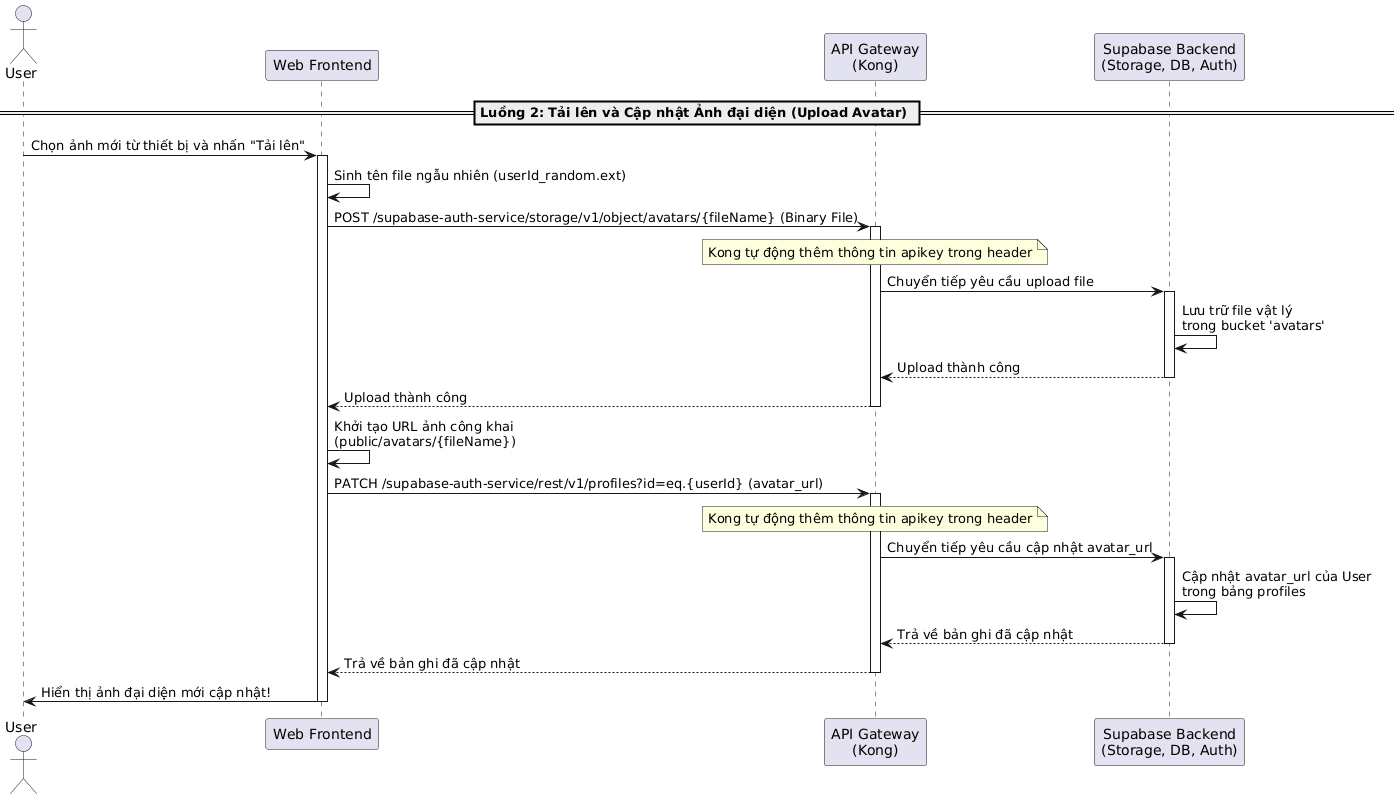
\includegraphics[scale = 0.2]{contents/Sequence/UML-Sequence-UserProfileUploadAvatar.png}
\caption{Sơ đồ tuần tự luồng Tải lên và Cập nhật Ảnh đại diện}
\end{figure}

\subparagraph{Các thành phần tham gia}

\begin{table}[H]
\centering
\renewcommand{\arraystretch}{1.3}

\begin{tabular}{|l|l|p{5cm}|}
\hline
\textbf{Thành phần} & \textbf{Phân loại} & \textbf{Vai trò trong hệ thống} \\ \hline
User & Actor & Người dùng thực hiện chọn ảnh và lưu ảnh đại diện mới. \\ \hline
Web Frontend & Component & Giao diện web Next.js. \\ \hline %%%% Component & Giao diện Next.js sinh tên tệp tin ngẫu nhiên, thực hiện tải ảnh và cập nhật địa chỉ ảnh mới vào hồ sơ. \\ \hline
API Gateway (Kong) & Component & Cổng API chuyển tiếp các yêu cầu API. \\ \hline %%%% Component & Định tuyến các yêu cầu liên quan tới Storage và PostgREST. \\ \hline
Supabase Backend & Component & Dịch vụ tích hợp quản lý lưu trữ tệp tin, CSDL và xác thực. \\ \hline
\end{tabular}
\caption{Các thành phần tham gia luồng Tải lên và Cập nhật Ảnh đại diện}
\end{table}

\subparagraph{Mô tả tổng quan}

\begin{itemize}
\item Người dùng tải tệp ảnh lên. Frontend sinh tên tệp tin (\texttt{userId\_random.ext}) rồi gửi tệp tin qua Gateway đến \texttt{Supabase Backend} để lưu trữ trong bucket \texttt{avatars} qua đường dẫn \texttt{/avatars/\{fileName\}}.
\item Sau khi tải lên thành công, Frontend khởi tạo đường dẫn ảnh công khai (\texttt{avatar\_url}) và thực hiện gửi yêu cầu \texttt{PATCH /profiles?id=eq.\{userId\}} qua Gateway để cập nhật thông tin ảnh đại diện của người dùng trong bảng \texttt{profiles} của Supabase Backend.
\end{itemize}
